\subsection{Conditioning on number of shots doesn't affect agents' performance}  \label{sec:results_conditioning}

Figure \ref{fig:k-conditioning} shows the score obtained by AdA for each percentile, in trial 1 of episodes with only 1 trial ($k=1$) and in trial 1 of episodes with 8 trials ($k=8$) in our held-out test set. The overlap of these lines indicates that AdA does not use the trial conditioning information it observes to adjust its behaviour in any way that affects its score. If the agent were to follow a more exploratory policy when it has more trials, we might expect the scores of trial 1 with $k=8$ to be lower than the score of trial 1 with $k=1$. 

This may be the optimal policy for our XLand 2.0 tasks, or it may reveal a limitation of our training procedure. One can imagine a scenario in which, knowing that there are $8$ trials in total, a Bayes-optimal policy chooses to display a less rewarding and more exploratory behaviour in trial $1$, compared to how it would behave if told that there was only a single trial in which to collect reward. For instance, an agent may be able to guarantee a deterministic reward later, having discovered some key information, at the cost of foregoing an stochastic reward early on. We did not directly incentivise this behaviour in our training process. In fact, we may have discouraged it, since AdA learns from all rewards in an episode (not just in the last trial), and with a discount factor smaller than 1, which could lead to myopic behaviour.  

\begin{figure}[t!]
    \centering
    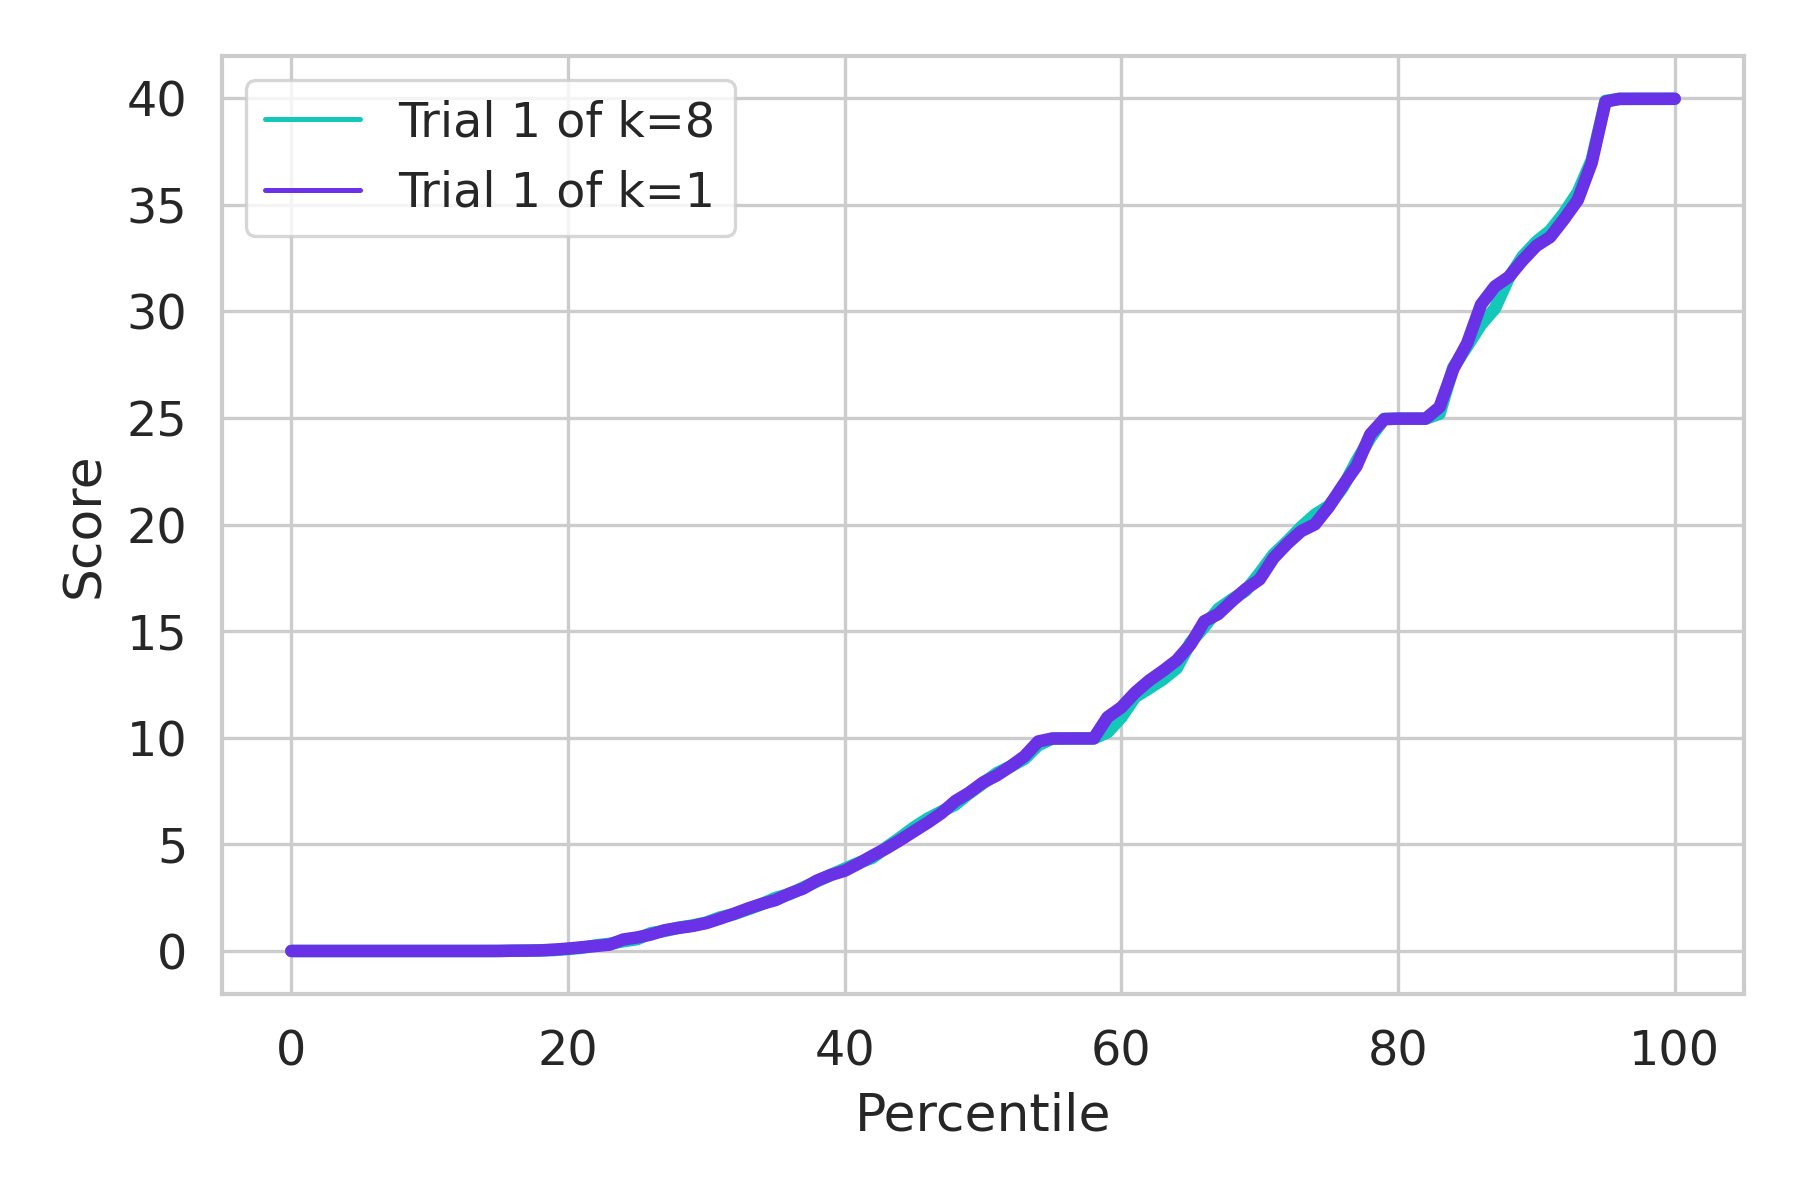
\includegraphics[width=0.5\linewidth]{figures/k-conditioning.png}

    \caption{A comparison of the first-trial score in episodes with 1 trial and episodes with 8 trials. The lines are almost perfectly overlapping, which indicates that our agent does not leverage number-of-trials conditioning information to adjust its policy to a more exploratory one in early trials when more trials are available.}
    \label{fig:k-conditioning}
\end{figure}